This section serves the testing of Hypothesis \ref{hpt:hypothesis_h} under
state of the global localisation art methods and CBGL, in varying environmental
conditions and sensor configurations. With regard to CBGL its three required
parameters were set to $(d_{\bm{l}},d_{\alpha},k) = (40, 2^5, 10)$ after
preparatory tests with the dataset tested against in subsection
\ref{subsec:exp_in_re_co}. The rationale of choosing appropriate
$d_{\bm{l}},d_{\alpha}$ is depicted in figure \ref{fig:a:determine_40_32}, and
$k$ was chosen as such in order to retain a high-enough true positive discovery
rate without significant increase in execution time (due to the application of
scan--to--map-scan matching on $k$ pose estimates).


\subsection{Experiments in real conditions}
\label{subsec:exp_in_re_co}

The first type of tests were conducted with the use of a Hokuyo UTM-30LX
sensor, whose angular range is $\lambda = 3\pi/2$ rad and maximum range
$r_{\max} = 30.0$ m, in the  Electrical and Computer Engineering Department's
Laboratory of Computer Systems Architecture (CSAL), Aristotle University of
Thessaloniki, Greece, a map of which is depicted in figure
\ref{fig:a:map_and_trajectory}. The sensor was mounted on a Robotnik RB1 robot,
which was teleoperated to move within the environment while range scans were
being captured. This resulted in $N_{S}=6669$ range scans, whose number of rays
were downsampled by a factor of four before being inputted to CBGL and ALS
\cite{als_jp}, an algorithm which implements Free-Space Features
\cite{als_eth}. CBGL's internal scan--to--map-scan matching method was chosen
to be PLICP \cite{Censi2008c} due to its low execution time and the scans'
non-panoramic field of view.  Other global localisation methods ?? were not to
tested for this type of experiment due to their infeasible execution time with
respect to the range dataset's volume. The top of figure \ref{fig:a:awesomeness}
depicts the proportion of output pose estimates from each method whose position
and orientation error was lower than varying values of outlier thresholds
$\delta_{\bm{l}}$, $\delta_{\theta}$; at the bottom they are depicted
exclusively with regard to CBGL's output and its internal pose sets. The mean
and standard deviation of the two methods' execution times were
$(\overline{\mu}_t^{\text{ALS}}, \sigma_t^{\text{ALS}}) = (6.15, 5.32)$ sec,
and $(\overline{\mu}_t^{\text{CBGL}}, \sigma_t^{\text{CBGL}}) = (1.61, 0.06)$
sec. From the experimental evidence it is clear that (a) hypothesis
\ref{hpt:hypothesis_h} is observed to be true $991$ times out of a thousand for
an outliers' locational threshold $\delta_{\bm{l}} = 0.5$ m when an angular
threshold is $\delta_{\theta}$ is not enforced, and (b) CBGL outperforms ALS in
terms of number of pose estimates within all locational and angular thresholds
and in terms of execution time.

\begin{figure}
  % GNUPLOT: LaTeX picture with Postscript
\begingroup
  \makeatletter
  \providecommand\color[2][]{%
    \GenericError{(gnuplot) \space\space\space\@spaces}{%
      Package color not loaded in conjunction with
      terminal option `colourtext'%
    }{See the gnuplot documentation for explanation.%
    }{Either use 'blacktext' in gnuplot or load the package
      color.sty in LaTeX.}%
    \renewcommand\color[2][]{}%
  }%
  \providecommand\includegraphics[2][]{%
    \GenericError{(gnuplot) \space\space\space\@spaces}{%
      Package graphicx or graphics not loaded%
    }{See the gnuplot documentation for explanation.%
    }{The gnuplot epslatex terminal needs graphicx.sty or graphics.sty.}%
    \renewcommand\includegraphics[2][]{}%
  }%
  \providecommand\rotatebox[2]{#2}%
  \@ifundefined{ifGPcolor}{%
    \newif\ifGPcolor
    \GPcolorfalse
  }{}%
  \@ifundefined{ifGPblacktext}{%
    \newif\ifGPblacktext
    \GPblacktexttrue
  }{}%
  % define a \g@addto@macro without @ in the name:
  \let\gplgaddtomacro\g@addto@macro
  % define empty templates for all commands taking text:
  \gdef\gplfronttext{}%
  \gdef\gplfronttext{}%
  \makeatother
  \ifGPblacktext
    % no textcolor at all
    \def\colorrgb#1{}%
    \def\colorgray#1{}%
  \else
    % gray or color?
    \ifGPcolor
      \def\colorrgb#1{\color[rgb]{#1}}%
      \def\colorgray#1{\color[gray]{#1}}%
      \expandafter\def\csname LTw\endcsname{\color{white}}%
      \expandafter\def\csname LTb\endcsname{\color{black}}%
      \expandafter\def\csname LTa\endcsname{\color{black}}%
      \expandafter\def\csname LT0\endcsname{\color[rgb]{1,0,0}}%
      \expandafter\def\csname LT1\endcsname{\color[rgb]{0,1,0}}%
      \expandafter\def\csname LT2\endcsname{\color[rgb]{0,0,1}}%
      \expandafter\def\csname LT3\endcsname{\color[rgb]{1,0,1}}%
      \expandafter\def\csname LT4\endcsname{\color[rgb]{0,1,1}}%
      \expandafter\def\csname LT5\endcsname{\color[rgb]{1,1,0}}%
      \expandafter\def\csname LT6\endcsname{\color[rgb]{0,0,0}}%
      \expandafter\def\csname LT7\endcsname{\color[rgb]{1,0.3,0}}%
      \expandafter\def\csname LT8\endcsname{\color[rgb]{0.5,0.5,0.5}}%
    \else
      % gray
      \def\colorrgb#1{\color{black}}%
      \def\colorgray#1{\color[gray]{#1}}%
      \expandafter\def\csname LTw\endcsname{\color{white}}%
      \expandafter\def\csname LTb\endcsname{\color{black}}%
      \expandafter\def\csname LTa\endcsname{\color{black}}%
      \expandafter\def\csname LT0\endcsname{\color{black}}%
      \expandafter\def\csname LT1\endcsname{\color{black}}%
      \expandafter\def\csname LT2\endcsname{\color{black}}%
      \expandafter\def\csname LT3\endcsname{\color{black}}%
      \expandafter\def\csname LT4\endcsname{\color{black}}%
      \expandafter\def\csname LT5\endcsname{\color{black}}%
      \expandafter\def\csname LT6\endcsname{\color{black}}%
      \expandafter\def\csname LT7\endcsname{\color{black}}%
      \expandafter\def\csname LT8\endcsname{\color{black}}%
    \fi
  \fi
    \setlength{\unitlength}{0.0500bp}%
    \ifx\gptboxheight\undefined%
      \newlength{\gptboxheight}%
      \newlength{\gptboxwidth}%
      \newsavebox{\gptboxtext}%
    \fi%
    \setlength{\fboxrule}{0.5pt}%
    \setlength{\fboxsep}{1pt}%
\begin{picture}(4500.00,4000.00)%
    \gplgaddtomacro\gplfronttext{%
      \colorrgb{0.15,0.15,0.15}%
      \put(318,2666){\makebox(0,0)[r]{\strut{}\footnotesize $0$}}%
      \colorrgb{0.15,0.15,0.15}%
      \put(318,2899){\makebox(0,0)[r]{\strut{}\footnotesize $500$}}%
      \colorrgb{0.15,0.15,0.15}%
      \put(318,3133){\makebox(0,0)[r]{\strut{}\footnotesize $1000$}}%
      \colorrgb{0.15,0.15,0.15}%
      \put(318,3366){\makebox(0,0)[r]{\strut{}\footnotesize $1500$}}%
      \colorrgb{0.15,0.15,0.15}%
      \put(318,3599){\makebox(0,0)[r]{\strut{}\footnotesize $2000$}}%
      \colorrgb{0.15,0.15,0.15}%
      \put(498,2566){\makebox(0,0){\strut{}\scriptsize $0$}}%
      \colorrgb{0.15,0.15,0.15}%
      \put(688,2566){\makebox(0,0){\strut{}\scriptsize $2$}}%
      \colorrgb{0.15,0.15,0.15}%
      \put(879,2566){\makebox(0,0){\strut{}\scriptsize $4$}}%
      \colorrgb{0.15,0.15,0.15}%
      \put(1070,2566){\makebox(0,0){\strut{}\scriptsize $6$}}%
      \colorrgb{0.15,0.15,0.15}%
      \put(1261,2566){\makebox(0,0){\strut{}\scriptsize $8$}}%
      \colorrgb{0.15,0.15,0.15}%
      \put(1451,2566){\makebox(0,0){\strut{}\scriptsize $10$}}%
    }%
    \gplgaddtomacro\gplfronttext{%
      \colorrgb{0.15,0.15,0.15}%
      \put(974,3716){\makebox(0,0){\strut{}\footnotesize $d_{\alpha} = 2^3$}}%
    }%
    \gplgaddtomacro\gplfronttext{%
      \colorrgb{0.15,0.15,0.15}%
      \put(1592,2666){\makebox(0,0)[r]{\strut{}}}%
      \colorrgb{0.15,0.15,0.15}%
      \put(1592,2899){\makebox(0,0)[r]{\strut{}}}%
      \colorrgb{0.15,0.15,0.15}%
      \put(1592,3133){\makebox(0,0)[r]{\strut{}}}%
      \colorrgb{0.15,0.15,0.15}%
      \put(1592,3366){\makebox(0,0)[r]{\strut{}}}%
      \colorrgb{0.15,0.15,0.15}%
      \put(1592,3599){\makebox(0,0)[r]{\strut{}}}%
      \colorrgb{0.15,0.15,0.15}%
      \put(1772,2566){\makebox(0,0){\strut{}\scriptsize $0$}}%
      \colorrgb{0.15,0.15,0.15}%
      \put(1963,2566){\makebox(0,0){\strut{}\scriptsize $2$}}%
      \colorrgb{0.15,0.15,0.15}%
      \put(2154,2566){\makebox(0,0){\strut{}\scriptsize $4$}}%
      \colorrgb{0.15,0.15,0.15}%
      \put(2356,2566){\makebox(0,0){\strut{}\scriptsize $6$}}%
      \colorrgb{0.15,0.15,0.15}%
      \put(2535,2566){\makebox(0,0){\strut{}\scriptsize $8$}}%
      \colorrgb{0.15,0.15,0.15}%
      \put(2726,2566){\makebox(0,0){\strut{}\scriptsize $10$}}%
    }%
    \gplgaddtomacro\gplfronttext{%
      \colorrgb{0.15,0.15,0.15}%
      \put(2249,3716){\makebox(0,0){\strut{}\footnotesize $d_{\alpha} = 2^4$}}%
    }%
    \gplgaddtomacro\gplfronttext{%
      \colorrgb{0.15,0.15,0.15}%
      \put(3048,2566){\makebox(0,0){\strut{}\scriptsize $0$}}%
      \colorrgb{0.15,0.15,0.15}%
      \put(3238,2566){\makebox(0,0){\strut{}\scriptsize $2$}}%
      \colorrgb{0.15,0.15,0.15}%
      \put(3429,2566){\makebox(0,0){\strut{}\scriptsize $4$}}%
      \colorrgb{0.15,0.15,0.15}%
      \put(3620,2566){\makebox(0,0){\strut{}\scriptsize $6$}}%
      \colorrgb{0.15,0.15,0.15}%
      \put(3811,2566){\makebox(0,0){\strut{}\scriptsize $8$}}%
      \colorrgb{0.15,0.15,0.15}%
      \put(4001,2566){\makebox(0,0){\strut{}\scriptsize $10$}}%
      \colorrgb{0.15,0.15,0.15}%
      \put(4181,2666){\makebox(0,0)[l]{\strut{}\footnotesize $0$}}%
      \colorrgb{0.15,0.15,0.15}%
      \put(4181,2899){\makebox(0,0)[l]{\strut{}\footnotesize $500$}}%
      \colorrgb{0.15,0.15,0.15}%
      \put(4181,3133){\makebox(0,0)[l]{\strut{}\footnotesize $1000$}}%
      \colorrgb{0.15,0.15,0.15}%
      \put(4181,3366){\makebox(0,0)[l]{\strut{}\footnotesize $1500$}}%
      \colorrgb{0.15,0.15,0.15}%
      \put(4181,3599){\makebox(0,0)[l]{\strut{}\footnotesize $2000$}}%
    }%
    \gplgaddtomacro\gplfronttext{%
      \colorrgb{0.15,0.15,0.15}%
      \put(4814,3132){\rotatebox{-90}{\makebox(0,0){\strut{}\footnotesize $d_{\bm{l}} = 40$}}}%
      \colorrgb{0.15,0.15,0.15}%
      \put(3524,3716){\makebox(0,0){\strut{}\footnotesize $d_{\alpha} = 2^5$}}%
    }%
    \gplgaddtomacro\gplfronttext{%
      \colorrgb{0.15,0.15,0.15}%
      \put(3048,1433){\makebox(0,0){\strut{}\scriptsize $0$}}%
      \colorrgb{0.15,0.15,0.15}%
      \put(3238,1433){\makebox(0,0){\strut{}\scriptsize $2$}}%
      \colorrgb{0.15,0.15,0.15}%
      \put(3429,1433){\makebox(0,0){\strut{}\scriptsize $4$}}%
      \colorrgb{0.15,0.15,0.15}%
      \put(3620,1433){\makebox(0,0){\strut{}\scriptsize $6$}}%
      \colorrgb{0.15,0.15,0.15}%
      \put(3811,1433){\makebox(0,0){\strut{}\scriptsize $8$}}%
      \colorrgb{0.15,0.15,0.15}%
      \put(4001,1433){\makebox(0,0){\strut{}\scriptsize $10$}}%
      \colorrgb{0.15,0.15,0.15}%
      \put(4181,1533){\makebox(0,0)[l]{\strut{}\footnotesize $0$}}%
      \colorrgb{0.15,0.15,0.15}%
      \put(4181,1766){\makebox(0,0)[l]{\strut{}\footnotesize $500$}}%
      \colorrgb{0.15,0.15,0.15}%
      \put(4181,2000){\makebox(0,0)[l]{\strut{}\footnotesize $1000$}}%
      \colorrgb{0.15,0.15,0.15}%
      \put(4181,2233){\makebox(0,0)[l]{\strut{}\footnotesize $1500$}}%
      \colorrgb{0.15,0.15,0.15}%
      \put(4181,2466){\makebox(0,0)[l]{\strut{}\footnotesize $2000$}}%
    }%
    \gplgaddtomacro\gplfronttext{%
      \colorrgb{0.15,0.15,0.15}%
      \put(4814,1999){\rotatebox{-90}{\makebox(0,0){\strut{}\footnotesize $d_{\bm{l}} = 20$}}}%
    }%
    \gplgaddtomacro\gplfronttext{%
      \colorrgb{0.15,0.15,0.15}%
      \put(3048,300){\makebox(0,0){\strut{}\scriptsize $0$}}%
      \colorrgb{0.15,0.15,0.15}%
      \put(3238,300){\makebox(0,0){\strut{}\scriptsize $2$}}%
      \colorrgb{0.15,0.15,0.15}%
      \put(3429,300){\makebox(0,0){\strut{}\scriptsize $4$}}%
      \colorrgb{0.15,0.15,0.15}%
      \put(3620,300){\makebox(0,0){\strut{}\scriptsize $6$}}%
      \colorrgb{0.15,0.15,0.15}%
      \put(3811,300){\makebox(0,0){\strut{}\scriptsize $8$}}%
      \colorrgb{0.15,0.15,0.15}%
      \put(4001,300){\makebox(0,0){\strut{}\scriptsize $10$}}%
      \colorrgb{0.15,0.15,0.15}%
      \put(4181,400){\makebox(0,0)[l]{\strut{}\footnotesize $0$}}%
      \colorrgb{0.15,0.15,0.15}%
      \put(4181,633){\makebox(0,0)[l]{\strut{}\footnotesize $500$}}%
      \colorrgb{0.15,0.15,0.15}%
      \put(4181,866){\makebox(0,0)[l]{\strut{}\footnotesize $1000$}}%
      \colorrgb{0.15,0.15,0.15}%
      \put(4181,1099){\makebox(0,0)[l]{\strut{}\footnotesize $1500$}}%
      \colorrgb{0.15,0.15,0.15}%
      \put(4181,1332){\makebox(0,0)[l]{\strut{}\footnotesize $2000$}}%
    }%
    \gplgaddtomacro\gplfronttext{%
      \colorrgb{0.15,0.15,0.15}%
      \put(4814,866){\rotatebox{-90}{\makebox(0,0){\strut{}\footnotesize $d_{\bm{l}} = 10$}}}%
    }%
    \gplgaddtomacro\gplfronttext{%
      \colorrgb{0.15,0.15,0.15}%
      \put(318,1533){\makebox(0,0)[r]{\strut{}\footnotesize $30\%$}}%
      \colorrgb{0.15,0.15,0.15}%
      \put(318,1844){\makebox(0,0)[r]{\strut{}\footnotesize $50\%$}}%
      \colorrgb{0.15,0.15,0.15}%
      \put(318,2155){\makebox(0,0)[r]{\strut{}\footnotesize $70\%$}}%
      \colorrgb{0.15,0.15,0.15}%
      \put(318,2466){\makebox(0,0)[r]{\strut{}\footnotesize $90\%$}}%
    }%
    \gplgaddtomacro\gplfronttext{%
      \colorrgb{0.15,0.15,0.15}%
      \put(1612,1433){\makebox(0,0){\strut{}\footnotesize Percent of inliers}}%
    }%
    \gplgaddtomacro\gplfronttext{%
      \colorrgb{0.15,0.15,0.15}%
      \put(318,400){\makebox(0,0)[r]{\strut{}\footnotesize $0.8$}}%
      \colorrgb{0.15,0.15,0.15}%
      \put(318,586){\makebox(0,0)[r]{\strut{}\footnotesize $1.0$}}%
      \colorrgb{0.15,0.15,0.15}%
      \put(318,773){\makebox(0,0)[r]{\strut{}\footnotesize $1.2$}}%
      \colorrgb{0.15,0.15,0.15}%
      \put(318,959){\makebox(0,0)[r]{\strut{}\footnotesize $1.4$}}%
      \colorrgb{0.15,0.15,0.15}%
      \put(318,1146){\makebox(0,0)[r]{\strut{}\footnotesize $1.6$}}%
      \colorrgb{0.15,0.15,0.15}%
      \put(318,1332){\makebox(0,0)[r]{\strut{}\footnotesize $1.8$}}%
    }%
    \gplgaddtomacro\gplfronttext{%
      \colorrgb{0.15,0.15,0.15}%
      \put(1612,300){\makebox(0,0){\strut{}\footnotesize Execution time [sec]}}%
    }%
    \put(0,0){\includegraphics{./figures/experiments/a/determine_40_32}}%
    \gplfronttext
  \end{picture}%
\endgroup

  \caption{\small Top row and right column: histograms of the number of times
           when exactly $n \in [0,k] = [0,10]$ pose estimates belonging to set
           $\mathcal{H}_1$ exhibited pose errors lower than $\delta =
           (\delta_{\bm{l}}^2 + \delta_{\theta}^2)^{1/2} =  (0.3^2 +
           0.4^2)^{1/2} = 0.5$ (m$^2$ + rad$^2$)$^{1/2}$. For densities
           $(d_{\bm{l}},d_{\alpha}) = (40, 2^5)$ this number is strictly
           increasing with $n$. Middle block: percent proportion of pose
           estimates whose pose error is lower than $\delta$ for varying field
           densities.  Bottom block: the corresponding execution times}
  \label{fig:a:determine_40_32}
\end{figure}


\begin{figure}
  % GNUPLOT: LaTeX picture with Postscript
\begingroup
  \makeatletter
  \providecommand\color[2][]{%
    \GenericError{(gnuplot) \space\space\space\@spaces}{%
      Package color not loaded in conjunction with
      terminal option `colourtext'%
    }{See the gnuplot documentation for explanation.%
    }{Either use 'blacktext' in gnuplot or load the package
      color.sty in LaTeX.}%
    \renewcommand\color[2][]{}%
  }%
  \providecommand\includegraphics[2][]{%
    \GenericError{(gnuplot) \space\space\space\@spaces}{%
      Package graphicx or graphics not loaded%
    }{See the gnuplot documentation for explanation.%
    }{The gnuplot epslatex terminal needs graphicx.sty or graphics.sty.}%
    \renewcommand\includegraphics[2][]{}%
  }%
  \providecommand\rotatebox[2]{#2}%
  \@ifundefined{ifGPcolor}{%
    \newif\ifGPcolor
    \GPcolorfalse
  }{}%
  \@ifundefined{ifGPblacktext}{%
    \newif\ifGPblacktext
    \GPblacktexttrue
  }{}%
  % define a \g@addto@macro without @ in the name:
  \let\gplgaddtomacro\g@addto@macro
  % define empty templates for all commands taking text:
  \gdef\gplfronttext{}%
  \gdef\gplfronttext{}%
  \makeatother
  \ifGPblacktext
    % no textcolor at all
    \def\colorrgb#1{}%
    \def\colorgray#1{}%
  \else
    % gray or color?
    \ifGPcolor
      \def\colorrgb#1{\color[rgb]{#1}}%
      \def\colorgray#1{\color[gray]{#1}}%
      \expandafter\def\csname LTw\endcsname{\color{white}}%
      \expandafter\def\csname LTb\endcsname{\color{black}}%
      \expandafter\def\csname LTa\endcsname{\color{black}}%
      \expandafter\def\csname LT0\endcsname{\color[rgb]{1,0,0}}%
      \expandafter\def\csname LT1\endcsname{\color[rgb]{0,1,0}}%
      \expandafter\def\csname LT2\endcsname{\color[rgb]{0,0,1}}%
      \expandafter\def\csname LT3\endcsname{\color[rgb]{1,0,1}}%
      \expandafter\def\csname LT4\endcsname{\color[rgb]{0,1,1}}%
      \expandafter\def\csname LT5\endcsname{\color[rgb]{1,1,0}}%
      \expandafter\def\csname LT6\endcsname{\color[rgb]{0,0,0}}%
      \expandafter\def\csname LT7\endcsname{\color[rgb]{1,0.3,0}}%
      \expandafter\def\csname LT8\endcsname{\color[rgb]{0.5,0.5,0.5}}%
    \else
      % gray
      \def\colorrgb#1{\color{black}}%
      \def\colorgray#1{\color[gray]{#1}}%
      \expandafter\def\csname LTw\endcsname{\color{white}}%
      \expandafter\def\csname LTb\endcsname{\color{black}}%
      \expandafter\def\csname LTa\endcsname{\color{black}}%
      \expandafter\def\csname LT0\endcsname{\color{black}}%
      \expandafter\def\csname LT1\endcsname{\color{black}}%
      \expandafter\def\csname LT2\endcsname{\color{black}}%
      \expandafter\def\csname LT3\endcsname{\color{black}}%
      \expandafter\def\csname LT4\endcsname{\color{black}}%
      \expandafter\def\csname LT5\endcsname{\color{black}}%
      \expandafter\def\csname LT6\endcsname{\color{black}}%
      \expandafter\def\csname LT7\endcsname{\color{black}}%
      \expandafter\def\csname LT8\endcsname{\color{black}}%
    \fi
  \fi
    \setlength{\unitlength}{0.0500bp}%
    \ifx\gptboxheight\undefined%
      \newlength{\gptboxheight}%
      \newlength{\gptboxwidth}%
      \newsavebox{\gptboxtext}%
    \fi%
    \setlength{\fboxrule}{0.5pt}%
    \setlength{\fboxsep}{1pt}%
\begin{picture}(5000.00,2500.00)%
    \gplgaddtomacro\gplfronttext{%
      \colorrgb{0.15,0.15,0.15}%
      \put(729,440){\makebox(0,0)[r]{\strut{}\footnotesize $-2.0$}}%
      \colorrgb{0.15,0.15,0.15}%
      \put(729,696){\makebox(0,0)[r]{\strut{}\footnotesize $0.0$}}%
      \colorrgb{0.15,0.15,0.15}%
      \put(729,953){\makebox(0,0)[r]{\strut{}\footnotesize $2.0$}}%
      \colorrgb{0.15,0.15,0.15}%
      \put(729,1209){\makebox(0,0)[r]{\strut{}\footnotesize $4.0$}}%
      \colorrgb{0.15,0.15,0.15}%
      \put(729,1466){\makebox(0,0)[r]{\strut{}\footnotesize $6.0$}}%
      \colorrgb{0.15,0.15,0.15}%
      \put(729,1722){\makebox(0,0)[r]{\strut{}\footnotesize $8.0$}}%
      \colorrgb{0.15,0.15,0.15}%
      \put(729,1979){\makebox(0,0)[r]{\strut{}\footnotesize $10.0$}}%
      \colorrgb{0.15,0.15,0.15}%
      \put(729,2235){\makebox(0,0)[r]{\strut{}\footnotesize $12.0$}}%
      \colorrgb{0.15,0.15,0.15}%
      \put(1310,220){\makebox(0,0){\strut{}\footnotesize $5.0$}}%
      \colorrgb{0.15,0.15,0.15}%
      \put(1951,220){\makebox(0,0){\strut{}\footnotesize $10.0$}}%
      \colorrgb{0.15,0.15,0.15}%
      \put(2592,220){\makebox(0,0){\strut{}\footnotesize $15.0$}}%
      \colorrgb{0.15,0.15,0.15}%
      \put(3233,220){\makebox(0,0){\strut{}\footnotesize $20.0$}}%
      \colorrgb{0.15,0.15,0.15}%
      \put(3874,220){\makebox(0,0){\strut{}\footnotesize $25.0$}}%
    }%
    \gplgaddtomacro\gplfronttext{%
    }%
    \put(0,0){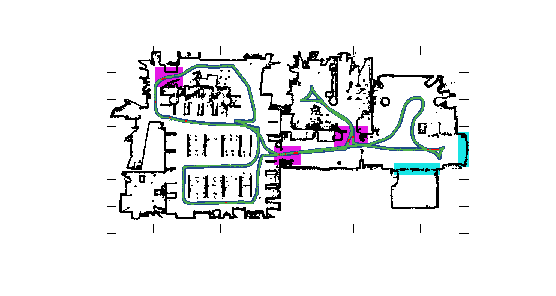
\includegraphics[trim={0 0 0 0.4cm},clip]{./figures/experiments/a/trajectory}}%
    \gplfronttext
  \end{picture}%
\endgroup

  \caption{\small The map of the CSAL environment (black), the trajectory of
           the sensor (blue), CBGL's estimated positions of the sensor (green),
           sensor poses for which CBGL estimated positions with error larger
           than $\delta_{\bm{l}} = 0.5$ m (red), and sources of great range
           noise (purple, cyan). Estimation is performed for each sensor pose
           independently of previous estimates or measurements}
           \label{fig:a:map_and_trajectory}
\end{figure}

\begin{figure}
  \definecolor{g1}{RGB}{200 200 200}
\definecolor{g2}{RGB}{162 162 162}
\definecolor{g3}{RGB}{137 137 137}
\definecolor{g4}{RGB}{77 175 74}

% GNUPLOT: LaTeX picture with Postscript
\begingroup
  \makeatletter
  \providecommand\color[2][]{%
    \GenericError{(gnuplot) \space\space\space\@spaces}{%
      Package color not loaded in conjunction with
      terminal option `colourtext'%
    }{See the gnuplot documentation for explanation.%
    }{Either use 'blacktext' in gnuplot or load the package
      color.sty in LaTeX.}%
    \renewcommand\color[2][]{}%
  }%
  \providecommand\includegraphics[2][]{%
    \GenericError{(gnuplot) \space\space\space\@spaces}{%
      Package graphicx or graphics not loaded%
    }{See the gnuplot documentation for explanation.%
    }{The gnuplot epslatex terminal needs graphicx.sty or graphics.sty.}%
    \renewcommand\includegraphics[2][]{}%
  }%
  \providecommand\rotatebox[2]{#2}%
  \@ifundefined{ifGPcolor}{%
    \newif\ifGPcolor
    \GPcolorfalse
  }{}%
  \@ifundefined{ifGPblacktext}{%
    \newif\ifGPblacktext
    \GPblacktexttrue
  }{}%
  % define a \g@addto@macro without @ in the name:
  \let\gplgaddtomacro\g@addto@macro
  % define empty templates for all commands taking text:
  \gdef\gplfronttext{}%
  \gdef\gplfronttext{}%
  \makeatother
  \ifGPblacktext
    % no textcolor at all
    \def\colorrgb#1{}%
    \def\colorgray#1{}%
  \else
    % gray or color?
    \ifGPcolor
      \def\colorrgb#1{\color[rgb]{#1}}%
      \def\colorgray#1{\color[gray]{#1}}%
      \expandafter\def\csname LTw\endcsname{\color{white}}%
      \expandafter\def\csname LTb\endcsname{\color{black}}%
      \expandafter\def\csname LTa\endcsname{\color{black}}%
      \expandafter\def\csname LT0\endcsname{\color[rgb]{1,0,0}}%
      \expandafter\def\csname LT1\endcsname{\color[rgb]{0,1,0}}%
      \expandafter\def\csname LT2\endcsname{\color[rgb]{0,0,1}}%
      \expandafter\def\csname LT3\endcsname{\color[rgb]{1,0,1}}%
      \expandafter\def\csname LT4\endcsname{\color[rgb]{0,1,1}}%
      \expandafter\def\csname LT5\endcsname{\color[rgb]{1,1,0}}%
      \expandafter\def\csname LT6\endcsname{\color[rgb]{0,0,0}}%
      \expandafter\def\csname LT7\endcsname{\color[rgb]{1,0.3,0}}%
      \expandafter\def\csname LT8\endcsname{\color[rgb]{0.5,0.5,0.5}}%
    \else
      % gray
      \def\colorrgb#1{\color{black}}%
      \def\colorgray#1{\color[gray]{#1}}%
      \expandafter\def\csname LTw\endcsname{\color{white}}%
      \expandafter\def\csname LTb\endcsname{\color{black}}%
      \expandafter\def\csname LTa\endcsname{\color{black}}%
      \expandafter\def\csname LT0\endcsname{\color{black}}%
      \expandafter\def\csname LT1\endcsname{\color{black}}%
      \expandafter\def\csname LT2\endcsname{\color{black}}%
      \expandafter\def\csname LT3\endcsname{\color{black}}%
      \expandafter\def\csname LT4\endcsname{\color{black}}%
      \expandafter\def\csname LT5\endcsname{\color{black}}%
      \expandafter\def\csname LT6\endcsname{\color{black}}%
      \expandafter\def\csname LT7\endcsname{\color{black}}%
      \expandafter\def\csname LT8\endcsname{\color{black}}%
    \fi
  \fi
    \setlength{\unitlength}{0.0500bp}%
    \ifx\gptboxheight\undefined%
      \newlength{\gptboxheight}%
      \newlength{\gptboxwidth}%
      \newsavebox{\gptboxtext}%
    \fi%
    \setlength{\fboxrule}{0.5pt}%
    \setlength{\fboxsep}{1pt}%
\begin{picture}(5000.00,2500.00)%
    \gplgaddtomacro\gplfronttext{%
      \colorrgb{0.15,0.15,0.15}%
      \put(1000,2600){\makebox(0,0){\strut{}{\color{g4}{\rule[0.6mm]{0.5cm}{0.5mm}}} \footnotesize Output}}
      \put(2500,2600){\makebox(0,0){\strut{}{\color{g3}{\rule[0.6mm]{0.5cm}{0.5mm}}} \footnotesize $\mathcal{H}_1[\arg \min f_{\psi}^{\bm{M}}(\mathcal{H}_2)]$}}
      \put(3900,2600){\makebox(0,0){\strut{}{\color{g2}{\rule[0.6mm]{0.5cm}{0.5mm}}} \footnotesize $\mathcal{H}_1$}}
      \put(4500,2600){\makebox(0,0){\strut{}{\color{g1}{\rule[0.6mm]{0.5cm}{0.5mm}}} \footnotesize $\mathcal{H}$}}
      \put(468,250){\makebox(0,0)[r]{\strut{}\footnotesize $0.0$}}%
      \colorrgb{0.15,0.15,0.15}%
      \put(468,750){\makebox(0,0)[r]{\strut{}\footnotesize $0.25$}}%
      \colorrgb{0.15,0.15,0.15}%
      \put(468,1250){\makebox(0,0)[r]{\strut{}\footnotesize $0.50$}}%
      \colorrgb{0.15,0.15,0.15}%
      \put(468,1793){\makebox(0,0)[r]{\strut{}\footnotesize $0.772$}}%
      \colorrgb{0.15,0.15,0.15}%
      \put(468,2105){\makebox(0,0)[r]{\strut{}\footnotesize $0.928$}}%
      \colorrgb{0.15,0.15,0.15}%
      \put(468,2231){\makebox(0,0)[r]{\strut{}\footnotesize $0.991$}}%
      \colorrgb{0.15,0.15,0.15}%
      \put(500,30){\makebox(0,0){\strut{}\footnotesize $5$\texttt{e}-$05$}}%
      \colorrgb{0.15,0.15,0.15}%
      \put(970,30){\makebox(0,0){\strut{}\footnotesize $0.01$}}%
      \colorrgb{0.15,0.15,0.15}%
      \put(1576,30){\makebox(0,0){\strut{}\footnotesize $0.50$}}%
      \colorrgb{0.15,0.15,0.15}%
      %\put(2040,30){\makebox(0,0){\strut{}\footnotesize $10.0$}}%
      \colorrgb{0.15,0.15,0.15}%
      \put(2199,30){\makebox(0,0){\strut{}\footnotesize $27.86$}}%
    }%
    \gplgaddtomacro\gplfronttext{%
      \colorrgb{0.15,0.15,0.15}%
      \put(1349,-300){\makebox(0,0){\strut{}\footnotesize Outliers locational threshold $\delta_{\bm{l}}$ [m]}}%
    }%
    \gplgaddtomacro\gplfronttext{%
      \colorrgb{0.15,0.15,0.15}%
      \put(2893,250){\makebox(0,0)[r]{\strut{}\footnotesize $0.0$}}%
      \colorrgb{0.15,0.15,0.15}%
      \put(2893,750){\makebox(0,0)[r]{\strut{}\footnotesize $0.25$}}%
      \colorrgb{0.15,0.15,0.15}%
      \put(2893,999){\makebox(0,0)[r]{\strut{}\footnotesize $0.375$}}%
      \colorrgb{0.15,0.15,0.15}%
      \put(2893,1153){\makebox(0,0)[r]{\strut{}\footnotesize $0.452$}}%
      \colorrgb{0.15,0.15,0.15}%
      \put(2893,2137){\makebox(0,0)[r]{\strut{}\footnotesize $0.944$}}%
      \colorrgb{0.15,0.15,0.15}%
      \put(2925,30){\makebox(0,0){\strut{}\footnotesize $4$\texttt{e}-$05$}}%
      \colorrgb{0.15,0.15,0.15}%
      \put(3740,30){\makebox(0,0){\strut{}\footnotesize $\frac{\pi}{1000}$}}%
      \colorrgb{0.15,0.15,0.15}%
      \put(4114,30){\makebox(0,0){\strut{}\footnotesize $\frac{\pi}{100}$}}%
      \colorrgb{0.15,0.15,0.15}%
      \put(4749,30){\makebox(0,0){\strut{}\footnotesize $\pi$}}%
    }%
    \gplgaddtomacro\gplfronttext{%
      \colorrgb{0.15,0.15,0.15}%
      \put(3837,-300){\makebox(0,0){\strut{}\footnotesize Outliers angular threshold $\delta_{\alpha}$ [rad]}}%
    }%
    \put(0,0){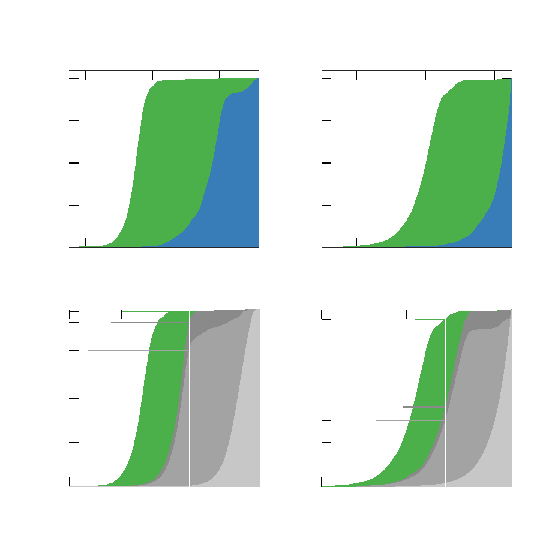
\includegraphics{./figures/experiments/a/awesomeness}}%
    \gplfronttext
  \end{picture}%
\endgroup

  \vspace{0.1cm}
  \caption{\small Proportions of pose estimates whose
           position and orientation error is lower than corresponding thresholds
           $\delta_{\bm{l}}$ and $\delta_{\theta}$. Top: ALS vs CBGL. Bottom:
           CBGL and internal pose estimate sets; the improvement in position
           and orientation induced by scan--to--map-scan matching is captured
           by the difference between the output (i.e.
           $\mathcal{H}_2[\arg \min f_{\psi}^{\bm{M}}(\mathcal{H}_2)]$) and
           $\mathcal{H}_1[\arg \min f_{\psi}^{\bm{M}}(\mathcal{H}_2)]$}
  \label{fig:a:awesomeness}
\end{figure}


\subsection{Simulations against sources of uncertainty}

\begin{figure}\hspace{0.5cm}
  \definecolor{c1}{RGB}{228,26,28}
\definecolor{c2}{RGB}{55,126,184}
\definecolor{c3}{RGB}{255,0,255}
\definecolor{c4}{RGB}{152,78,163}
\definecolor{c5}{RGB}{255,127,0}
\definecolor{c6}{RGB}{77,175,74}
\hspace{0.5cm}

% GNUPLOT: LaTeX picture with Postscript
\begingroup
  \makeatletter
  \providecommand\color[2][]{%
    \GenericError{(gnuplot) \space\space\space\@spaces}{%
      Package color not loaded in conjunction with
      terminal option `colourtext'%
    }{See the gnuplot documentation for explanation.%
    }{Either use 'blacktext' in gnuplot or load the package
      color.sty in LaTeX.}%
    \renewcommand\color[2][]{}%
  }%
  \providecommand\includegraphics[2][]{%
    \GenericError{(gnuplot) \space\space\space\@spaces}{%
      Package graphicx or graphics not loaded%
    }{See the gnuplot documentation for explanation.%
    }{The gnuplot epslatex terminal needs graphicx.sty or graphics.sty.}%
    \renewcommand\includegraphics[2][]{}%
  }%
  \providecommand\rotatebox[2]{#2}%
  \@ifundefined{ifGPcolor}{%
    \newif\ifGPcolor
    \GPcolorfalse
  }{}%
  \@ifundefined{ifGPblacktext}{%
    \newif\ifGPblacktext
    \GPblacktexttrue
  }{}%
  % define a \g@addto@macro without @ in the name:
  \let\gplgaddtomacro\g@addto@macro
  % define empty templates for all commands taking text:
  \gdef\gplfronttext{}%
  \gdef\gplfronttext{}%
  \makeatother
  \ifGPblacktext
    % no textcolor at all
    \def\colorrgb#1{}%
    \def\colorgray#1{}%
  \else
    % gray or color?
    \ifGPcolor
      \def\colorrgb#1{\color[rgb]{#1}}%
      \def\colorgray#1{\color[gray]{#1}}%
      \expandafter\def\csname LTw\endcsname{\color{white}}%
      \expandafter\def\csname LTb\endcsname{\color{black}}%
      \expandafter\def\csname LTa\endcsname{\color{black}}%
      \expandafter\def\csname LT0\endcsname{\color[rgb]{1,0,0}}%
      \expandafter\def\csname LT1\endcsname{\color[rgb]{0,1,0}}%
      \expandafter\def\csname LT2\endcsname{\color[rgb]{0,0,1}}%
      \expandafter\def\csname LT3\endcsname{\color[rgb]{1,0,1}}%
      \expandafter\def\csname LT4\endcsname{\color[rgb]{0,1,1}}%
      \expandafter\def\csname LT5\endcsname{\color[rgb]{1,1,0}}%
      \expandafter\def\csname LT6\endcsname{\color[rgb]{0,0,0}}%
      \expandafter\def\csname LT7\endcsname{\color[rgb]{1,0.3,0}}%
      \expandafter\def\csname LT8\endcsname{\color[rgb]{0.5,0.5,0.5}}%
    \else
      % gray
      \def\colorrgb#1{\color{black}}%
      \def\colorgray#1{\color[gray]{#1}}%
      \expandafter\def\csname LTw\endcsname{\color{white}}%
      \expandafter\def\csname LTb\endcsname{\color{black}}%
      \expandafter\def\csname LTa\endcsname{\color{black}}%
      \expandafter\def\csname LT0\endcsname{\color{black}}%
      \expandafter\def\csname LT1\endcsname{\color{black}}%
      \expandafter\def\csname LT2\endcsname{\color{black}}%
      \expandafter\def\csname LT3\endcsname{\color{black}}%
      \expandafter\def\csname LT4\endcsname{\color{black}}%
      \expandafter\def\csname LT5\endcsname{\color{black}}%
      \expandafter\def\csname LT6\endcsname{\color{black}}%
      \expandafter\def\csname LT7\endcsname{\color{black}}%
      \expandafter\def\csname LT8\endcsname{\color{black}}%
    \fi
  \fi
    \setlength{\unitlength}{0.0500bp}%
    \ifx\gptboxheight\undefined%
      \newlength{\gptboxheight}%
      \newlength{\gptboxwidth}%
      \newsavebox{\gptboxtext}%
    \fi%
    \setlength{\fboxrule}{0.5pt}%
    \setlength{\fboxsep}{1pt}%
  \hspace{0.5cm}
\begin{picture}(5000.00,3000.00)%
    \gplgaddtomacro\gplfronttext{%
      \colorrgb{0.15,0.15,0.15}%
      \put(368,1724){\makebox(0,0)[r]{\strut{}\footnotesize $0\%$}}%
      \colorrgb{0.15,0.15,0.15}%
      \put(368,1968){\makebox(0,0)[r]{\strut{}\footnotesize $25\%$}}%
      \colorrgb{0.15,0.15,0.15}%
      \put(368,2212){\makebox(0,0)[r]{\strut{}\footnotesize $50\%$}}%
      \colorrgb{0.15,0.15,0.15}%
      \put(368,2455){\makebox(0,0)[r]{\strut{}\footnotesize $75\%$}}%
      \colorrgb{0.15,0.15,0.15}%
      \put(368,2699){\makebox(0,0)[r]{\strut{}\footnotesize $100\%$}}%
      \colorrgb{0.15,0.15,0.15}%
      \put(833,1504){\makebox(0,0){\strut{}\footnotesize $\bm{p}_a^W$}}%
      \colorrgb{0.15,0.15,0.15}%
      \put(1500,1504){\makebox(0,0){\strut{}\footnotesize $\bm{p}_b^W$}}%
      \colorrgb{0.15,0.15,0.15}%
      \put(2166,1504){\makebox(0,0){\strut{}\footnotesize $\bm{p}_c^W$}}%
      \colorrgb{0.15,0.15,0.15}%
      \put(2833,1504){\makebox(0,0){\strut{}\footnotesize $\bm{p}_d^W$}}%
      \colorrgb{0.15,0.15,0.15}%
      \put(3499,1504){\makebox(0,0){\strut{}\footnotesize $\bm{p}_f^W$}}%
      \colorrgb{0.15,0.15,0.15}%
      \put(4166,1504){\makebox(0,0){\strut{}\footnotesize $\bm{p}_g^W$}}%
    }%
    \gplgaddtomacro\gplfronttext{%
      \colorrgb{0.15,0.15,0.15}%
      \put(-198,2211){\rotatebox{90}{\makebox(0,0){\strut{}\footnotesize WAREHOUSE}}}%
      \put( 200,3000){\makebox(0,0){\strut{}{\color{c1}{\rule[0.6mm]{0.3cm}{0.5mm}}} \scriptsize MCL}}
      \put( 800,3000){\makebox(0,0){\strut{}{\color{c2}{\rule[0.6mm]{0.3cm}{0.5mm}}} \scriptsize ALS}}
      \put(1450,3000){\makebox(0,0){\strut{}{\color{c3}{\rule[0.6mm]{0.3cm}{0.5mm}}} \scriptsize GMCL}}
      \put(2300,3000){\makebox(0,0){\strut{}{\color{c4}{\rule[0.6mm]{0.3cm}{0.5mm}}} \scriptsize PGL-FMIC}}
      \put(3300,3000){\makebox(0,0){\strut{}{\color{c5}{\rule[0.6mm]{0.3cm}{0.5mm}}} \scriptsize PGL-PLICP}}
      \put(4250,3000){\makebox(0,0){\strut{}{\color{c6}{\rule[0.6mm]{0.3cm}{0.5mm}}} \scriptsize CBGL}}
    }%
    \gplgaddtomacro\gplfronttext{%
      \colorrgb{0.15,0.15,0.15}%
      \put(368,300){\makebox(0,0)[r]{\strut{}\footnotesize $0\%$}}%
      \colorrgb{0.15,0.15,0.15}%
      \put(368,544){\makebox(0,0)[r]{\strut{}\footnotesize $25\%$}}%
      \colorrgb{0.15,0.15,0.15}%
      \put(368,787){\makebox(0,0)[r]{\strut{}\footnotesize $50\%$}}%
      \colorrgb{0.15,0.15,0.15}%
      \put(368,1031){\makebox(0,0)[r]{\strut{}\footnotesize $75\%$}}%
      \colorrgb{0.15,0.15,0.15}%
      \put(368,1274){\makebox(0,0)[r]{\strut{}\footnotesize $100\%$}}%
      \colorrgb{0.15,0.15,0.15}%
      \put(700,80){\makebox(0,0){\strut{}\footnotesize $\bm{p}_a^G$}}%
      \colorrgb{0.15,0.15,0.15}%
      \put(1100,80){\makebox(0,0){\strut{}\footnotesize $\bm{p}_b^G$}}%
      \colorrgb{0.15,0.15,0.15}%
      \put(1500,80){\makebox(0,0){\strut{}\footnotesize $\bm{p}_c^G$}}%
      \colorrgb{0.15,0.15,0.15}%
      \put(1900,80){\makebox(0,0){\strut{}\footnotesize $\bm{p}_d^G$}}%
      \colorrgb{0.15,0.15,0.15}%
      \put(2300,80){\makebox(0,0){\strut{}\footnotesize $\bm{p}_e^G$}}%
      \colorrgb{0.15,0.15,0.15}%
      \put(2699,80){\makebox(0,0){\strut{}\footnotesize $\bm{p}_f^G$}}%
      \colorrgb{0.15,0.15,0.15}%
      \put(3099,80){\makebox(0,0){\strut{}\footnotesize $\bm{p}_g^G$}}%
      \colorrgb{0.15,0.15,0.15}%
      \put(3499,80){\makebox(0,0){\strut{}\footnotesize $\bm{p}_h^G$}}%
      \colorrgb{0.15,0.15,0.15}%
      \put(3899,80){\makebox(0,0){\strut{}\footnotesize $\bm{p}_i^G$}}%
      \colorrgb{0.15,0.15,0.15}%
      \put(4299,80){\makebox(0,0){\strut{}\footnotesize $\bm{p}_j^G$}}%
    }%
    \gplgaddtomacro\gplfronttext{%
      \colorrgb{0.15,0.15,0.15}%
      \put(-198,787){\rotatebox{90}{\makebox(0,0){\strut{}\footnotesize WILLOWGARAGE}}}%
    }%
    \put(0,0){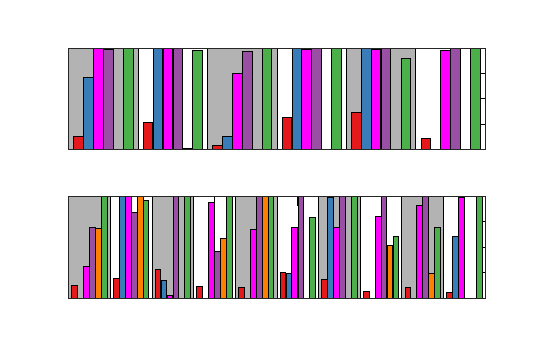
\includegraphics{./figures/experiments/b/inliers_per_pose}}%
    \gplfronttext
  \end{picture}%
\endgroup

  \caption{\small}
  \label{fig:}
\end{figure}
%\begin{figure}
  %\input{./figures/experiments/b/outliers.tex}
  %\caption{\small}
  %\label{fig:}
%\end{figure}
\begin{figure}
  \definecolor{c1}{RGB}{228,26,28}
\definecolor{c2}{RGB}{55,126,184}
\definecolor{c3}{RGB}{255,0,255}
\definecolor{c4}{RGB}{152,78,163}
\definecolor{c5}{RGB}{255,127,0}
\definecolor{c6}{RGB}{77,175,74}

% GNUPLOT: LaTeX picture with Postscript
\begingroup
  \makeatletter
  \providecommand\color[2][]{%
    \GenericError{(gnuplot) \space\space\space\@spaces}{%
      Package color not loaded in conjunction with
      terminal option `colourtext'%
    }{See the gnuplot documentation for explanation.%
    }{Either use 'blacktext' in gnuplot or load the package
      color.sty in LaTeX.}%
    \renewcommand\color[2][]{}%
  }%
  \providecommand\includegraphics[2][]{%
    \GenericError{(gnuplot) \space\space\space\@spaces}{%
      Package graphicx or graphics not loaded%
    }{See the gnuplot documentation for explanation.%
    }{The gnuplot epslatex terminal needs graphicx.sty or graphics.sty.}%
    \renewcommand\includegraphics[2][]{}%
  }%
  \providecommand\rotatebox[2]{#2}%
  \@ifundefined{ifGPcolor}{%
    \newif\ifGPcolor
    \GPcolorfalse
  }{}%
  \@ifundefined{ifGPblacktext}{%
    \newif\ifGPblacktext
    \GPblacktexttrue
  }{}%
  % define a \g@addto@macro without @ in the name:
  \let\gplgaddtomacro\g@addto@macro
  % define empty templates for all commands taking text:
  \gdef\gplfronttext{}%
  \gdef\gplfronttext{}%
  \makeatother
  \ifGPblacktext
    % no textcolor at all
    \def\colorrgb#1{}%
    \def\colorgray#1{}%
  \else
    % gray or color?
    \ifGPcolor
      \def\colorrgb#1{\color[rgb]{#1}}%
      \def\colorgray#1{\color[gray]{#1}}%
      \expandafter\def\csname LTw\endcsname{\color{white}}%
      \expandafter\def\csname LTb\endcsname{\color{black}}%
      \expandafter\def\csname LTa\endcsname{\color{black}}%
      \expandafter\def\csname LT0\endcsname{\color[rgb]{1,0,0}}%
      \expandafter\def\csname LT1\endcsname{\color[rgb]{0,1,0}}%
      \expandafter\def\csname LT2\endcsname{\color[rgb]{0,0,1}}%
      \expandafter\def\csname LT3\endcsname{\color[rgb]{1,0,1}}%
      \expandafter\def\csname LT4\endcsname{\color[rgb]{0,1,1}}%
      \expandafter\def\csname LT5\endcsname{\color[rgb]{1,1,0}}%
      \expandafter\def\csname LT6\endcsname{\color[rgb]{0,0,0}}%
      \expandafter\def\csname LT7\endcsname{\color[rgb]{1,0.3,0}}%
      \expandafter\def\csname LT8\endcsname{\color[rgb]{0.5,0.5,0.5}}%
    \else
      % gray
      \def\colorrgb#1{\color{black}}%
      \def\colorgray#1{\color[gray]{#1}}%
      \expandafter\def\csname LTw\endcsname{\color{white}}%
      \expandafter\def\csname LTb\endcsname{\color{black}}%
      \expandafter\def\csname LTa\endcsname{\color{black}}%
      \expandafter\def\csname LT0\endcsname{\color{black}}%
      \expandafter\def\csname LT1\endcsname{\color{black}}%
      \expandafter\def\csname LT2\endcsname{\color{black}}%
      \expandafter\def\csname LT3\endcsname{\color{black}}%
      \expandafter\def\csname LT4\endcsname{\color{black}}%
      \expandafter\def\csname LT5\endcsname{\color{black}}%
      \expandafter\def\csname LT6\endcsname{\color{black}}%
      \expandafter\def\csname LT7\endcsname{\color{black}}%
      \expandafter\def\csname LT8\endcsname{\color{black}}%
    \fi
  \fi
    \setlength{\unitlength}{0.0500bp}%
    \ifx\gptboxheight\undefined%
      \newlength{\gptboxheight}%
      \newlength{\gptboxwidth}%
      \newsavebox{\gptboxtext}%
    \fi%
    \setlength{\fboxrule}{0.5pt}%
    \setlength{\fboxsep}{1pt}%
\begin{picture}(5000.00,1500.00)%
    \gplgaddtomacro\gplfronttext{%
      \colorrgb{0.15,0.15,0.15}%
      \put(368,267){\makebox(0,0)[r]{\strut{}\footnotesize $10^{0}$}}%
      \colorrgb{0.15,0.15,0.15}%
      \put(368,657){\makebox(0,0)[r]{\strut{}\footnotesize $10^{1}$}}%
      \colorrgb{0.15,0.15,0.15}%
      \put(368,1046){\makebox(0,0)[r]{\strut{}\footnotesize $10^{2}$}}%
    }%
    \gplgaddtomacro\gplfronttext{%
      \colorrgb{0.15,0.15,0.15}%
      \put(1474,-70){\makebox(0,0){\strut{}\footnotesize WAREHOUSE}}%
      \put( 400,1500){\makebox(0,0){\strut{}{\color{c1}{\rule[0.6mm]{0.3cm}{0.5mm}}} \scriptsize MCL}}
      \put(1000,1500){\makebox(0,0){\strut{}{\color{c2}{\rule[0.6mm]{0.3cm}{0.5mm}}} \scriptsize ALS}}
      \put(1650,1500){\makebox(0,0){\strut{}{\color{c3}{\rule[0.6mm]{0.3cm}{0.5mm}}} \scriptsize GMCL}}
      \put(2500,1500){\makebox(0,0){\strut{}{\color{c4}{\rule[0.6mm]{0.3cm}{0.5mm}}} \scriptsize PGL-FMIC}}
      \put(3500,1500){\makebox(0,0){\strut{}{\color{c5}{\rule[0.6mm]{0.3cm}{0.5mm}}} \scriptsize PGL-PLICP}}
      \put(4450,1500){\makebox(0,0){\strut{}{\color{c6}{\rule[0.6mm]{0.3cm}{0.5mm}}} \scriptsize CBGL}}
    }%
    \gplgaddtomacro\gplfronttext{%
      \colorrgb{0.15,0.15,0.15}%
      \put(2418,267){\makebox(0,0)[r]{\strut{}\footnotesize $10^{0}$}}%
      \colorrgb{0.15,0.15,0.15}%
      \put(2418,657){\makebox(0,0)[r]{\strut{}\footnotesize $10^{1}$}}%
      \colorrgb{0.15,0.15,0.15}%
      \put(2418,1046){\makebox(0,0)[r]{\strut{}\footnotesize $10^{2}$}}%
    }%
    \gplgaddtomacro\gplfronttext{%
      \colorrgb{0.15,0.15,0.15}%
      \put(3524,-70){\makebox(0,0){\strut{}\footnotesize WILLOWGARAGE}}%
    }%
    \put(0,0){\includegraphics{./figures/experiments/b/exec_times}}%
    \gplfronttext
  \end{picture}%
\endgroup

  \caption{\small}
  \label{fig:}
\end{figure}


\subsection{Simulations against environment disparity and choice of scan--to--map-scan matching methods}
\begin{figure}
  % GNUPLOT: LaTeX picture with Postscript
\begingroup
  \makeatletter
  \providecommand\color[2][]{%
    \GenericError{(gnuplot) \space\space\space\@spaces}{%
      Package color not loaded in conjunction with
      terminal option `colourtext'%
    }{See the gnuplot documentation for explanation.%
    }{Either use 'blacktext' in gnuplot or load the package
      color.sty in LaTeX.}%
    \renewcommand\color[2][]{}%
  }%
  \providecommand\includegraphics[2][]{%
    \GenericError{(gnuplot) \space\space\space\@spaces}{%
      Package graphicx or graphics not loaded%
    }{See the gnuplot documentation for explanation.%
    }{The gnuplot epslatex terminal needs graphicx.sty or graphics.sty.}%
    \renewcommand\includegraphics[2][]{}%
  }%
  \providecommand\rotatebox[2]{#2}%
  \@ifundefined{ifGPcolor}{%
    \newif\ifGPcolor
    \GPcolorfalse
  }{}%
  \@ifundefined{ifGPblacktext}{%
    \newif\ifGPblacktext
    \GPblacktexttrue
  }{}%
  % define a \g@addto@macro without @ in the name:
  \let\gplgaddtomacro\g@addto@macro
  % define empty templates for all commands taking text:
  \gdef\gplfronttext{}%
  \gdef\gplfronttext{}%
  \makeatother
  \ifGPblacktext
    % no textcolor at all
    \def\colorrgb#1{}%
    \def\colorgray#1{}%
  \else
    % gray or color?
    \ifGPcolor
      \def\colorrgb#1{\color[rgb]{#1}}%
      \def\colorgray#1{\color[gray]{#1}}%
      \expandafter\def\csname LTw\endcsname{\color{white}}%
      \expandafter\def\csname LTb\endcsname{\color{black}}%
      \expandafter\def\csname LTa\endcsname{\color{black}}%
      \expandafter\def\csname LT0\endcsname{\color[rgb]{1,0,0}}%
      \expandafter\def\csname LT1\endcsname{\color[rgb]{0,1,0}}%
      \expandafter\def\csname LT2\endcsname{\color[rgb]{0,0,1}}%
      \expandafter\def\csname LT3\endcsname{\color[rgb]{1,0,1}}%
      \expandafter\def\csname LT4\endcsname{\color[rgb]{0,1,1}}%
      \expandafter\def\csname LT5\endcsname{\color[rgb]{1,1,0}}%
      \expandafter\def\csname LT6\endcsname{\color[rgb]{0,0,0}}%
      \expandafter\def\csname LT7\endcsname{\color[rgb]{1,0.3,0}}%
      \expandafter\def\csname LT8\endcsname{\color[rgb]{0.5,0.5,0.5}}%
    \else
      % gray
      \def\colorrgb#1{\color{black}}%
      \def\colorgray#1{\color[gray]{#1}}%
      \expandafter\def\csname LTw\endcsname{\color{white}}%
      \expandafter\def\csname LTb\endcsname{\color{black}}%
      \expandafter\def\csname LTa\endcsname{\color{black}}%
      \expandafter\def\csname LT0\endcsname{\color{black}}%
      \expandafter\def\csname LT1\endcsname{\color{black}}%
      \expandafter\def\csname LT2\endcsname{\color{black}}%
      \expandafter\def\csname LT3\endcsname{\color{black}}%
      \expandafter\def\csname LT4\endcsname{\color{black}}%
      \expandafter\def\csname LT5\endcsname{\color{black}}%
      \expandafter\def\csname LT6\endcsname{\color{black}}%
      \expandafter\def\csname LT7\endcsname{\color{black}}%
      \expandafter\def\csname LT8\endcsname{\color{black}}%
    \fi
  \fi
    \setlength{\unitlength}{0.0500bp}%
    \ifx\gptboxheight\undefined%
      \newlength{\gptboxheight}%
      \newlength{\gptboxwidth}%
      \newsavebox{\gptboxtext}%
    \fi%
    \setlength{\fboxrule}{0.5pt}%
    \setlength{\fboxsep}{1pt}%
\begin{picture}(5000.00,2500.00)%
    \gplgaddtomacro\gplfronttext{%
      \colorrgb{0.15,0.15,0.15}%
      \put(368,250){\makebox(0,0)[r]{\strut{}0}}%
      \colorrgb{0.15,0.15,0.15}%
      \put(368,650){\makebox(0,0)[r]{\strut{}0.2}}%
      \colorrgb{0.15,0.15,0.15}%
      \put(368,1050){\makebox(0,0)[r]{\strut{}0.4}}%
      \colorrgb{0.15,0.15,0.15}%
      \put(368,1449){\makebox(0,0)[r]{\strut{}0.6}}%
      \colorrgb{0.15,0.15,0.15}%
      \put(368,1849){\makebox(0,0)[r]{\strut{}0.8}}%
      \colorrgb{0.15,0.15,0.15}%
      \put(368,2249){\makebox(0,0)[r]{\strut{}1}}%
      \colorrgb{0.15,0.15,0.15}%
      \put(826,30){\makebox(0,0){\strut{}$10^{-2}$}}%
      \colorrgb{0.15,0.15,0.15}%
      \put(1200,30){\makebox(0,0){\strut{}$10^{-1}$}}%
      \colorrgb{0.15,0.15,0.15}%
      \put(1575,30){\makebox(0,0){\strut{}$10^{0}$}}%
      \colorrgb{0.15,0.15,0.15}%
      \put(1949,30){\makebox(0,0){\strut{}$10^{1}$}}%
      \colorrgb{0.15,0.15,0.15}%
      \put(2323,30){\makebox(0,0){\strut{}$10^{2}$}}%
    }%
    \gplgaddtomacro\gplfronttext{%
    }%
    \gplgaddtomacro\gplfronttext{%
      \colorrgb{0.15,0.15,0.15}%
      \put(2493,250){\makebox(0,0)[r]{\strut{}0}}%
      \colorrgb{0.15,0.15,0.15}%
      \put(2493,650){\makebox(0,0)[r]{\strut{}0.2}}%
      \colorrgb{0.15,0.15,0.15}%
      \put(2493,1050){\makebox(0,0)[r]{\strut{}0.4}}%
      \colorrgb{0.15,0.15,0.15}%
      \put(2493,1449){\makebox(0,0)[r]{\strut{}0.6}}%
      \colorrgb{0.15,0.15,0.15}%
      \put(2493,1849){\makebox(0,0)[r]{\strut{}0.8}}%
      \colorrgb{0.15,0.15,0.15}%
      \put(2493,2249){\makebox(0,0)[r]{\strut{}1}}%
      \colorrgb{0.15,0.15,0.15}%
      \put(2813,30){\makebox(0,0){\strut{}$10^{-4}$}}%
      \colorrgb{0.15,0.15,0.15}%
      \put(3188,30){\makebox(0,0){\strut{}$10^{-3}$}}%
      \colorrgb{0.15,0.15,0.15}%
      \put(3563,30){\makebox(0,0){\strut{}$10^{-2}$}}%
      \colorrgb{0.15,0.15,0.15}%
      \put(3938,30){\makebox(0,0){\strut{}$10^{-1}$}}%
      \colorrgb{0.15,0.15,0.15}%
      \put(4313,30){\makebox(0,0){\strut{}$10^{0}$}}%
    }%
    \gplgaddtomacro\gplfronttext{%
    }%
    \put(0,0){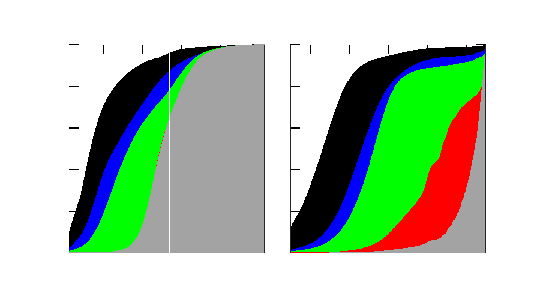
\includegraphics{./figures/experiments/c/awesome}}%
    \gplfronttext
  \end{picture}%
\endgroup

  \caption{\small}
  \label{fig:}
\end{figure}
\begin{figure}
  \definecolor{c0}{RGB}{162 162 162}
\definecolor{c1}{RGB}{102 194 165}
\definecolor{c2}{RGB}{252 141 98}
\definecolor{c3}{RGB}{41 160 203}
\definecolor{c4}{RGB}{231 138 195}

% GNUPLOT: LaTeX picture with Postscript
\begingroup
  \makeatletter
  \providecommand\color[2][]{%
    \GenericError{(gnuplot) \space\space\space\@spaces}{%
      Package color not loaded in conjunction with
      terminal option `colourtext'%
    }{See the gnuplot documentation for explanation.%
    }{Either use 'blacktext' in gnuplot or load the package
      color.sty in LaTeX.}%
    \renewcommand\color[2][]{}%
  }%
  \providecommand\includegraphics[2][]{%
    \GenericError{(gnuplot) \space\space\space\@spaces}{%
      Package graphicx or graphics not loaded%
    }{See the gnuplot documentation for explanation.%
    }{The gnuplot epslatex terminal needs graphicx.sty or graphics.sty.}%
    \renewcommand\includegraphics[2][]{}%
  }%
  \providecommand\rotatebox[2]{#2}%
  \@ifundefined{ifGPcolor}{%
    \newif\ifGPcolor
    \GPcolorfalse
  }{}%
  \@ifundefined{ifGPblacktext}{%
    \newif\ifGPblacktext
    \GPblacktexttrue
  }{}%
  % define a \g@addto@macro without @ in the name:
  \let\gplgaddtomacro\g@addto@macro
  % define empty templates for all commands taking text:
  \gdef\gplfronttext{}%
  \gdef\gplfronttext{}%
  \makeatother
  \ifGPblacktext
    % no textcolor at all
    \def\colorrgb#1{}%
    \def\colorgray#1{}%
  \else
    % gray or color?
    \ifGPcolor
      \def\colorrgb#1{\color[rgb]{#1}}%
      \def\colorgray#1{\color[gray]{#1}}%
      \expandafter\def\csname LTw\endcsname{\color{white}}%
      \expandafter\def\csname LTb\endcsname{\color{black}}%
      \expandafter\def\csname LTa\endcsname{\color{black}}%
      \expandafter\def\csname LT0\endcsname{\color[rgb]{1,0,0}}%
      \expandafter\def\csname LT1\endcsname{\color[rgb]{0,1,0}}%
      \expandafter\def\csname LT2\endcsname{\color[rgb]{0,0,1}}%
      \expandafter\def\csname LT3\endcsname{\color[rgb]{1,0,1}}%
      \expandafter\def\csname LT4\endcsname{\color[rgb]{0,1,1}}%
      \expandafter\def\csname LT5\endcsname{\color[rgb]{1,1,0}}%
      \expandafter\def\csname LT6\endcsname{\color[rgb]{0,0,0}}%
      \expandafter\def\csname LT7\endcsname{\color[rgb]{1,0.3,0}}%
      \expandafter\def\csname LT8\endcsname{\color[rgb]{0.5,0.5,0.5}}%
    \else
      % gray
      \def\colorrgb#1{\color{black}}%
      \def\colorgray#1{\color[gray]{#1}}%
      \expandafter\def\csname LTw\endcsname{\color{white}}%
      \expandafter\def\csname LTb\endcsname{\color{black}}%
      \expandafter\def\csname LTa\endcsname{\color{black}}%
      \expandafter\def\csname LT0\endcsname{\color{black}}%
      \expandafter\def\csname LT1\endcsname{\color{black}}%
      \expandafter\def\csname LT2\endcsname{\color{black}}%
      \expandafter\def\csname LT3\endcsname{\color{black}}%
      \expandafter\def\csname LT4\endcsname{\color{black}}%
      \expandafter\def\csname LT5\endcsname{\color{black}}%
      \expandafter\def\csname LT6\endcsname{\color{black}}%
      \expandafter\def\csname LT7\endcsname{\color{black}}%
      \expandafter\def\csname LT8\endcsname{\color{black}}%
    \fi
  \fi
    \setlength{\unitlength}{0.0500bp}%
    \ifx\gptboxheight\undefined%
      \newlength{\gptboxheight}%
      \newlength{\gptboxwidth}%
      \newsavebox{\gptboxtext}%
    \fi%
    \setlength{\fboxrule}{0.5pt}%
    \setlength{\fboxsep}{1pt}%
\begin{picture}(5000.00,1500.00)%
    \gplgaddtomacro\gplfronttext{%
      \colorrgb{0.15,0.15,0.15}%
      \put(468,224){\makebox(0,0)[r]{\strut{}\scriptsize $10^{-4}$}}%
      \colorrgb{0.15,0.15,0.15}%
      \put(468,468){\makebox(0,0)[r]{\strut{}\scriptsize $10^{-3}$}}%
      \colorrgb{0.15,0.15,0.15}%
      \put(468,713){\makebox(0,0)[r]{\strut{}\scriptsize $10^{-2}$}}%
      \colorrgb{0.15,0.15,0.15}%
      \put(468,957){\makebox(0,0)[r]{\strut{}\scriptsize $10^{-1}$}}%
      \colorrgb{0.15,0.15,0.15}%
      \put(368,1202){\makebox(0,0)[r]{\strut{}\scriptsize $10^{0}$}}%
    }%
    \gplgaddtomacro\gplfronttext{%
      \colorrgb{0.15,0.15,0.15}%
      \put(999,-70){\makebox(0,0){\strut{}\scriptsize Position errors [m]}}%
      \put( 800,1500){\makebox(0,0){\strut{}{\color{c0}{\rule[0.6mm]{0.3cm}{0.5mm}}} \scriptsize $\mathcal{H}_1$}}
      \put( 1400,1500){\makebox(0,0){\strut{}{\color{c1}{\rule[0.6mm]{0.3cm}{0.5mm}}} \scriptsize NDT}}
      \put(2300,1500){\makebox(0,0){\strut{}{\color{c2}{\rule[0.6mm]{0.3cm}{0.5mm}}} \scriptsize FastGICP}}
      \put(3400,1500){\makebox(0,0){\strut{}{\color{c3}{\rule[0.6mm]{0.3cm}{0.5mm}}} \scriptsize FastVGICP}}
      \put(4200,1500){\makebox(0,0){\strut{}{\color{c4}{\rule[0.6mm]{0.3cm}{0.5mm}}} \scriptsize \texttt{x1}}}
    }%
    \gplgaddtomacro\gplfronttext{%
      \colorrgb{0.15,0.15,0.15}%
      \put(1968,210){\makebox(0,0)[r]{\strut{}\scriptsize $10^{-4}$}}%
      \colorrgb{0.15,0.15,0.15}%
      \put(1968,410){\makebox(0,0)[r]{\strut{}\scriptsize $10^{-5}$}}%
      \colorrgb{0.15,0.15,0.15}%
      \put(1968,610){\makebox(0,0)[r]{\strut{}\scriptsize $10^{-3}$}}%
      \colorrgb{0.15,0.15,0.15}%
      \put(1968,810){\makebox(0,0)[r]{\strut{}\scriptsize $10^{-2}$}}%
      \colorrgb{0.15,0.15,0.15}%
      \put(1968,1009){\makebox(0,0)[r]{\strut{}\scriptsize $10^{-1}$}}%
      \colorrgb{0.15,0.15,0.15}%
      \put(1868,1209){\makebox(0,0)[r]{\strut{}\scriptsize $10^{0}$}}%
    }%
    \gplgaddtomacro\gplfronttext{%
      \colorrgb{0.15,0.15,0.15}%
      \put(2499,-70){\makebox(0,0){\strut{}\scriptsize Orientation errors [rad]}}%
    }%
    \gplgaddtomacro\gplfronttext{%
      \colorrgb{0.15,0.15,0.15}%
      \put(3468,150){\makebox(0,0)[r]{\strut{}\scriptsize $0.0$}}%
      \colorrgb{0.15,0.15,0.15}%
      \put(3468,450){\makebox(0,0)[r]{\strut{}\scriptsize $2.0$}}%
      \colorrgb{0.15,0.15,0.15}%
      \put(3468,750){\makebox(0,0)[r]{\strut{}\scriptsize $4.0$}}%
      \colorrgb{0.15,0.15,0.15}%
      \put(3468,1049){\makebox(0,0)[r]{\strut{}\scriptsize $6.0$}}%
      \colorrgb{0.15,0.15,0.15}%
      \put(3468,1349){\makebox(0,0)[r]{\strut{}\scriptsize $8.0$}}%
    }%
    \gplgaddtomacro\gplfronttext{%
      \colorrgb{0.15,0.15,0.15}%
      \put(3999,-70){\makebox(0,0){\strut{}\scriptsize Execution times [sec]}}%
    }%
    \put(0,0){\includegraphics{./figures/experiments/c/errors}}%
    \gplfronttext
  \end{picture}%
\endgroup

  \caption{\small}
  \label{fig:}
\end{figure}

